\newcommand{\TeamNo}{31}

\newcommand{\HWno}{05}

\newcommand{\AuthorOneName}{Merve Nur Öztürk}
\newcommand{\AuthorOneID}{2311322}

\newcommand{\AuthorTwoName}{Atakan Süslü}
\newcommand{\AuthorTwoID}{2311371}

\newcommand{\AuthorThreeName}{Betül Rana Kuran}
\newcommand{\AuthorThreeID}{2311173}


\documentclass[letterpaper,12pt]{article}
\usepackage{tabularx} % extra features for tabular environment
\usepackage{amsmath}  % improve math presentation
\usepackage{amssymb}
\usepackage{xcolor}
\usepackage{float}
\usepackage[export]{adjustbox}
\usepackage{graphicx} % takes care of graphic including machinery
\usepackage[margin=1in,letterpaper]{geometry} % decreases margins
\usepackage{cite} % takes care of citations

\begin{document}
\begin{center}
AE 305, 2020-21 Fall \hfill \textbf{HW \HWno} \hfill \textbf{Team \TeamNo} \\
\noindent\rule{\textwidth}{0.4pt}
\begin{tabular}{p{0.33\textwidth} | p{0.33\textwidth} | p{0.33\textwidth} }
	\AuthorOneName&\AuthorTwoName&\AuthorThreeName\\
	\textit{\AuthorOneID}&\textit{\AuthorTwoID}&\textit{\AuthorThreeID}
\end{tabular}
\noindent\rule{\textwidth}{0.4pt}
\end{center}

%Report start

\section{Introduction}
Elliptic partial differential equations can be solved by using finite difference equations,
and the most common FDE for the solution of an elliptic PDE is obtained by second-order
central difference approximations of the derivatives. Afterwards, the FDE can
be solved either by direct solution methods or iterative methods. In this homework, a 2D
heat equation is given:

\begin{equation}
	\frac{\partial^2T}{\partial x^2} + \frac{\partial^2T}{\partial y^2} = 0
	\label{eqn:heateqn}
\end{equation}

It is requested to compute the steady state temperature distribution on a given 2D model
of a room having a width of 10m and a height of 6m by solving the above equation for 
two different cases, one is with a radiator and the other is without a radiator. First,
the iterative methods are used; Point Jacobi, Gauss-Seidel, SOR and Line Gauss-Seidel
methods, then the solution is obtained by the direct solution methods. For the final
solution, it is asked to plot the heat flux distribution in the room, and the heat flux
vector is given as follows:

\begin{equation}
	\vec{q} = -k \nabla T
	\label{eqn:heatflux}
\end{equation}

It is also asked to compare the convergence rates of the iterative methods.
\section{Method}
FDE of the governing equation of this homework (Equation \ref{eqn:heateqn}) is obtained by second-order central difference approximations of the derivatives.
\begin{equation}
	\frac{T_{i+1,j}-2T_{i,j}+T_{i-1,j}}{\Delta x^2}+\frac{T_{i,j+1}-2T_{i,j}+T_{i,j-1}}{\Delta y^2}
	\label{eqn:fde}
\end{equation}
When $i$ and $j$ coincide with the boundries of the room or the radiator, they are excluded
from the solution of the heat equation since at these points the temperatures are equal to
temperatures of the boundries.\\
When $\beta = \frac{\Delta x}{\Delta y}$ substituted into Equation \ref{eqn:fde}, equation becomes:
\begin{eqnarray}
	T_{i+1,j}-2T_{i,j}+T_{i-1,j}+\beta ^2(T_{i,j+1}-2T_{i,j}+T_{i,j-1})&=&0 \nonumber \\
	\beta^2T_{i,j-1}+T_{i-1,j}-2(1+\beta^2)T_{i,j}+T_{i+1,j}+\beta ^2T_{i,j+1}&=&0 
	\label{eqn:basic}
\end{eqnarray}
This five-point formula gives the system of linear algebraic equations, which can be solved by two methods,
namely direct solution methods and iterative solution methods.
\subsection{Direct Solution Method}
\subsubsection{Gauss Elimination}
In this homework, Gauss elimination method is used as direct solution method. The system of linear
equations formed by five-point formula (Equation \ref{eqn:basic}).
\begin{equation}
	aT_{i-1,j}+bT_{i,j}+cT_{i+1,j}+dT_{i,j-1}+eT_{i,j+1}=0
\end{equation}
with Dirichlet typ BCs, the system of equations can be writen in $\underline{A}\mbox{ }\underline{T}=\underline{f}$ form
where $\underline{A}$ is coefficient matrix.
\begin{equation}
	a_i x_{i-1}+b_i x_i+c_i x_{i+1}=f_i
\end{equation}
\begin{equation}
	\begin{bmatrix}
		b     & c    & 0    &\dots & e   &\dots &0    &\dots &\dots&\dots \\
		a     & b    & c    &0    &\dots &e     & 0   &\dots &\dots&\dots \\
		0     & a    & b    &c    & 0   &\dots &e    &0    &\dots&\dots \\
		\vdots&    & a    &b    & c   & 0    &\dots &e    &0    &\dots \\
		d     & 0    & a    &b    & c   & 0    &\dots &\dots &e    &\dots \\
		0     & d    & a    &b    & c   & 0    &\dots &\dots &\dots &e     \\
		0     & 0    &\ddots &a    & c   & 0    &\dots &\dots &\dots &e      
		\end{bmatrix}
	\begin{Bmatrix}
		x_1\\
		x_2\\
		\vdots\\
		x_{k-1}\\
		x_k
		\end{Bmatrix}
	=
	\begin{Bmatrix}
		f_1\\
		f_2\\
		\vdots\\
		f_{k-1}\\
		f_k
	\end{Bmatrix}
	\label{eqn:matrx}
\end{equation}

\subsection{Iterative Solution Methods}
\subsubsection{Point Iterative Methods}
\paragraph{Point Jacobi Iteration}
In this method, every terms in Equation \ref{eqn:basic} are kept at $k$
where $k$ is denoted as iteration level except $T_{i,j}$. $T_{i,j}$ which is kept
at new iteration level $k+1$. Then equation becomes:
\begin{equation}
	T_{i,j}^{k+1}=\frac{1}{2(1+\beta^2)}[T_{i-1,j}^{k}+T_{i+1,j}^{k}+\beta ^2(T_{i,j-1}^{k}+T_{i,j+1}^{k})]
\label{eqn:jacobi}
\end{equation}
where $k$ corresponds previous calculated values or initial guess at the start
of iteration process of $T$ values over the room except boundary conditions.
\paragraph{Gauss-Seidel Iteration}
Differently from Point Jacobi method, in Gauss-Seidel method, the unknown dependent
variable values of Equation \ref{eqn:basic} are used as soon as they become available
at the $k+1$ iteration level.
\begin{equation}
	T_{i,j}^{k+1}=\frac{1}{2(1+\beta^2)}[T_{i-1,j}^{k+1}+T_{i+1,j}^{k}+\beta ^2(T_{i,j-1}^{k+1}+T_{i,j+1}^{k})]
\label{eqn:gs}
\end{equation}
\paragraph{Successive Over-Relaxation Method}
In this method, the convergence of solution is can be accelerated by multiplying the relaxation
parameter, $\omega$, with the amount of the change in each step. First, $T_{i,j}^k$ is substracted
from the Gauss-Seidel iteration method to obtain $\Delta T$.
\begin{equation}
	T_{i,j}^{k+1}\vert_{GS}-T_{i,j}^{k}=\Delta T\vert{GS}=\frac{1}{2(1+\beta^2)}[T_{i-1,j}^{k+1}+T_{i+1,j}^{k}+\beta ^2(T_{i,j-1}^{k+1}+T_{i,j+1}^{k})]-T_{i,j}^{k}
\label{eqn:sor1}
\end{equation}
Then, $\Delta T$ is multiplied by $\omega$
\begin{eqnarray}
	T_{i,j}^{k+1}\vert_{SOR}&=&T_{i,j}^{k}+\omega\Delta T\vert{GS} \nonumber \\
	&=&(1-\omega)T_{i,j}^{k}+\frac{\omega}{2(1+\beta^2)}[T_{i-1,j}^{k+1}+T_{i+1,j}^{k}+\beta^2(T_{i,j-1}^{k+1}+T_{i,j+1}^{k})]
	\label{eqn:sor}
\end{eqnarray}
To obtain convergent solutions, relaxatation parameter,$\omega$, is chosen in (0,2) interval.
The optimum value of $\omega$ can be determined by numerical experimentations. If $\omega$ is chosen in
(0,1) interval, under-relaxation occurs, which prevents the divegence by slowing the convergence for the solution of
certain non-linear partial derivative equations.
\subsubsection{Line Iterations}
\paragraph{Line Gauss-Seidel Method} In this method, iterations are made line by line, in one direction. One more term of Equation
\ref{eqn:gs} is expressed at $k+1$ iteration level. Then, equation becomes:
\begin{equation}
	T_{i,j}^{k+1}=\frac{1}{2(1+\beta^2)}[T_{i-1,j}^{k+1}+T_{i+1,j}^{k+1}+\beta ^2(T_{i,j-1}^{k+1}+T_{i,j+1}^{k})]
\end{equation}
To make iteration line by line, j is kept constant. Therefore, every $T_{ ,j}$ term should be in left
hand side of the equation.
\begin{equation}
	T_{i-1,j}^{k+1}-2(1+\beta^2)T_{i,j}^{k+1}+T_{i+1,j}^{k+1}=-\beta^2(T_{i,j+1}^{k}+T_{i,j-1}^{k+1})]
\label{eqn:lgs}
\end{equation}
For constant j grid lines, Equation \ref{eqn:lgs} is applied to all i's. The
system of linear equations which includes tridiagonal coefficient matrix is formed. Its
convergence rate is higher than the Gauss-Seidel method. On the other hand, a system of equations
is solved every iterations;hence, in each iteration, it requires more computations.
The effect of BCs at i=0 and i=imax is instantly visible in the solution.
\newpage
\section{Results and Discussion}

\subsection{Solution of the Heat Equation in the Absence of a Radiator}
Figures \ref{fig:pointnorad}, \ref{fig:gaussnorad}, and \ref{fig:sornorad}
illustrates the solution of the heat equation by using Point Jacobi, Gauss-Seidel,
and SOR methods, respectively. As can be seen from these figures, all the solutions
with different methods converged to approximately the same heat flux distributions.
In all solutions, flux vectors have the same directions, which are from the walls
with higher temperature to the wall with the lower temperature perpendicularly.
Moreover, near the insulated wall, these flux vectors are parallel and the temperature
contours are perpendicular to the wall since the temperature gradient is zero at the
insulated wall. Therefore, there is no heat transfer across the insulated wall. 

\begin{figure}[H] 
	\centering 
	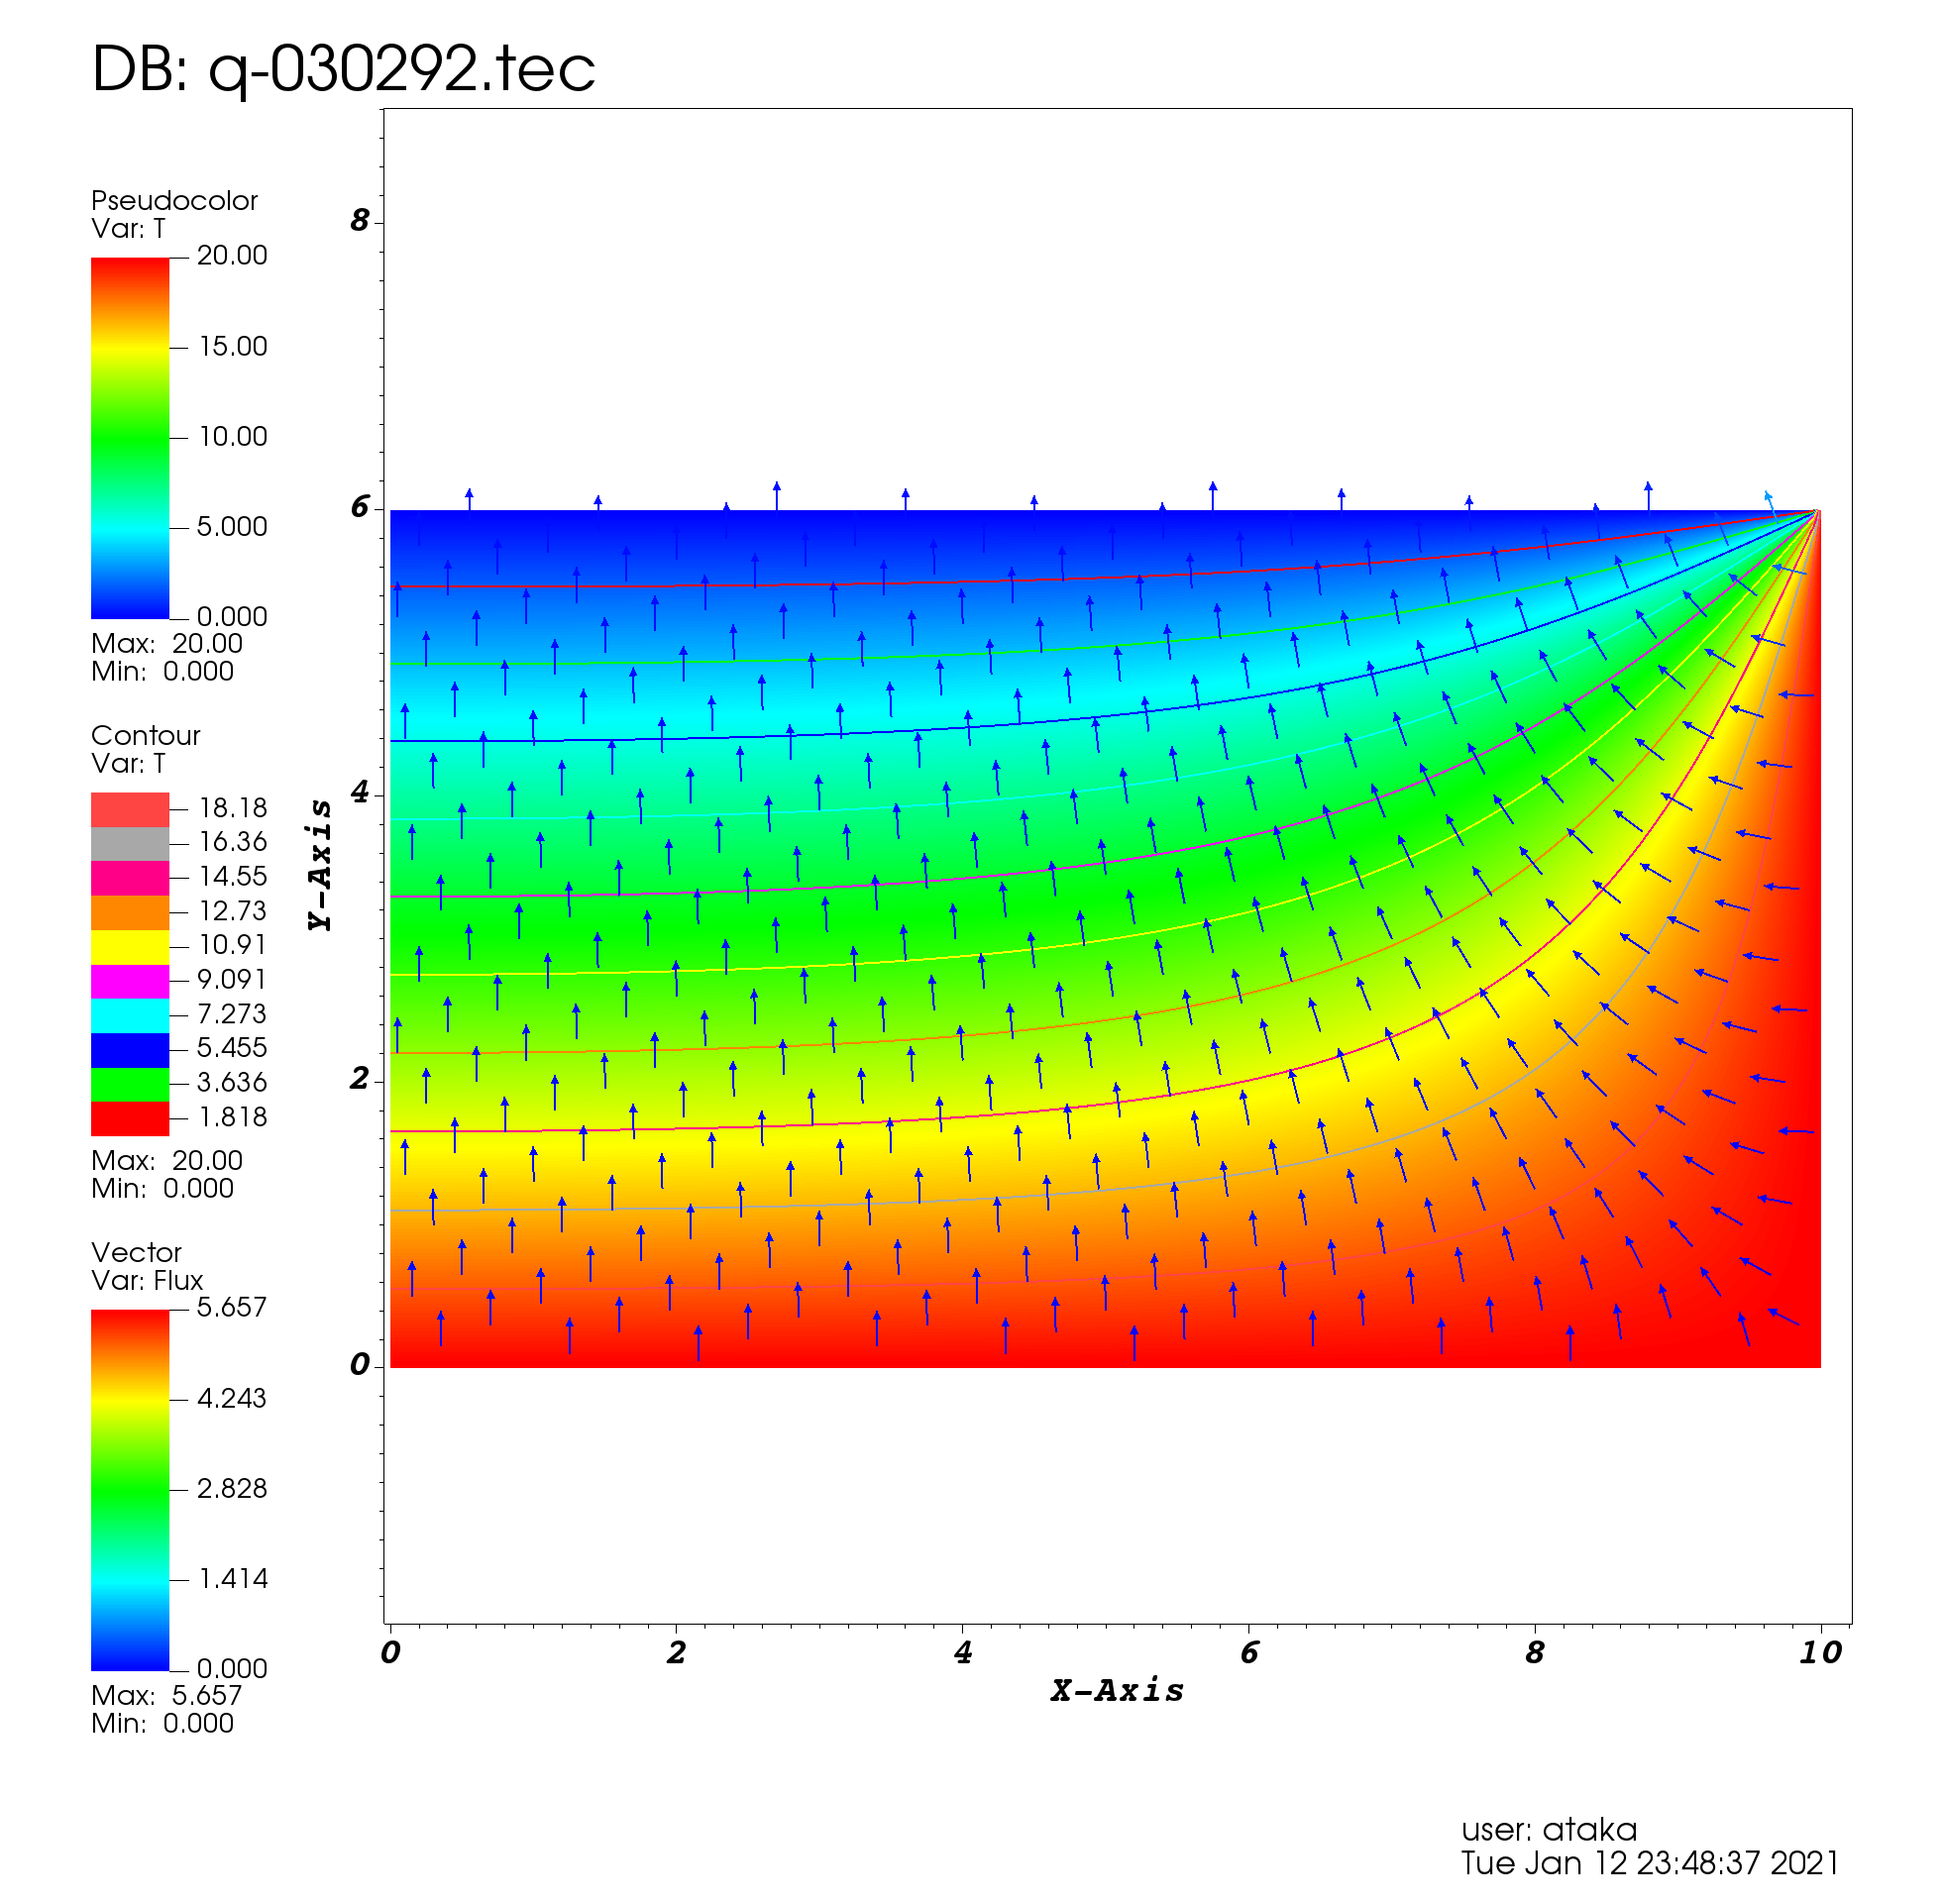
\includegraphics[max height=12cm]{graphs/point_norad/point_norad.png}
	\caption{Solution of the heat equation by Point Jacobi method.}
 	\label{fig:pointnorad}
\end{figure}
\begin{figure}[H] 
	\centering 
	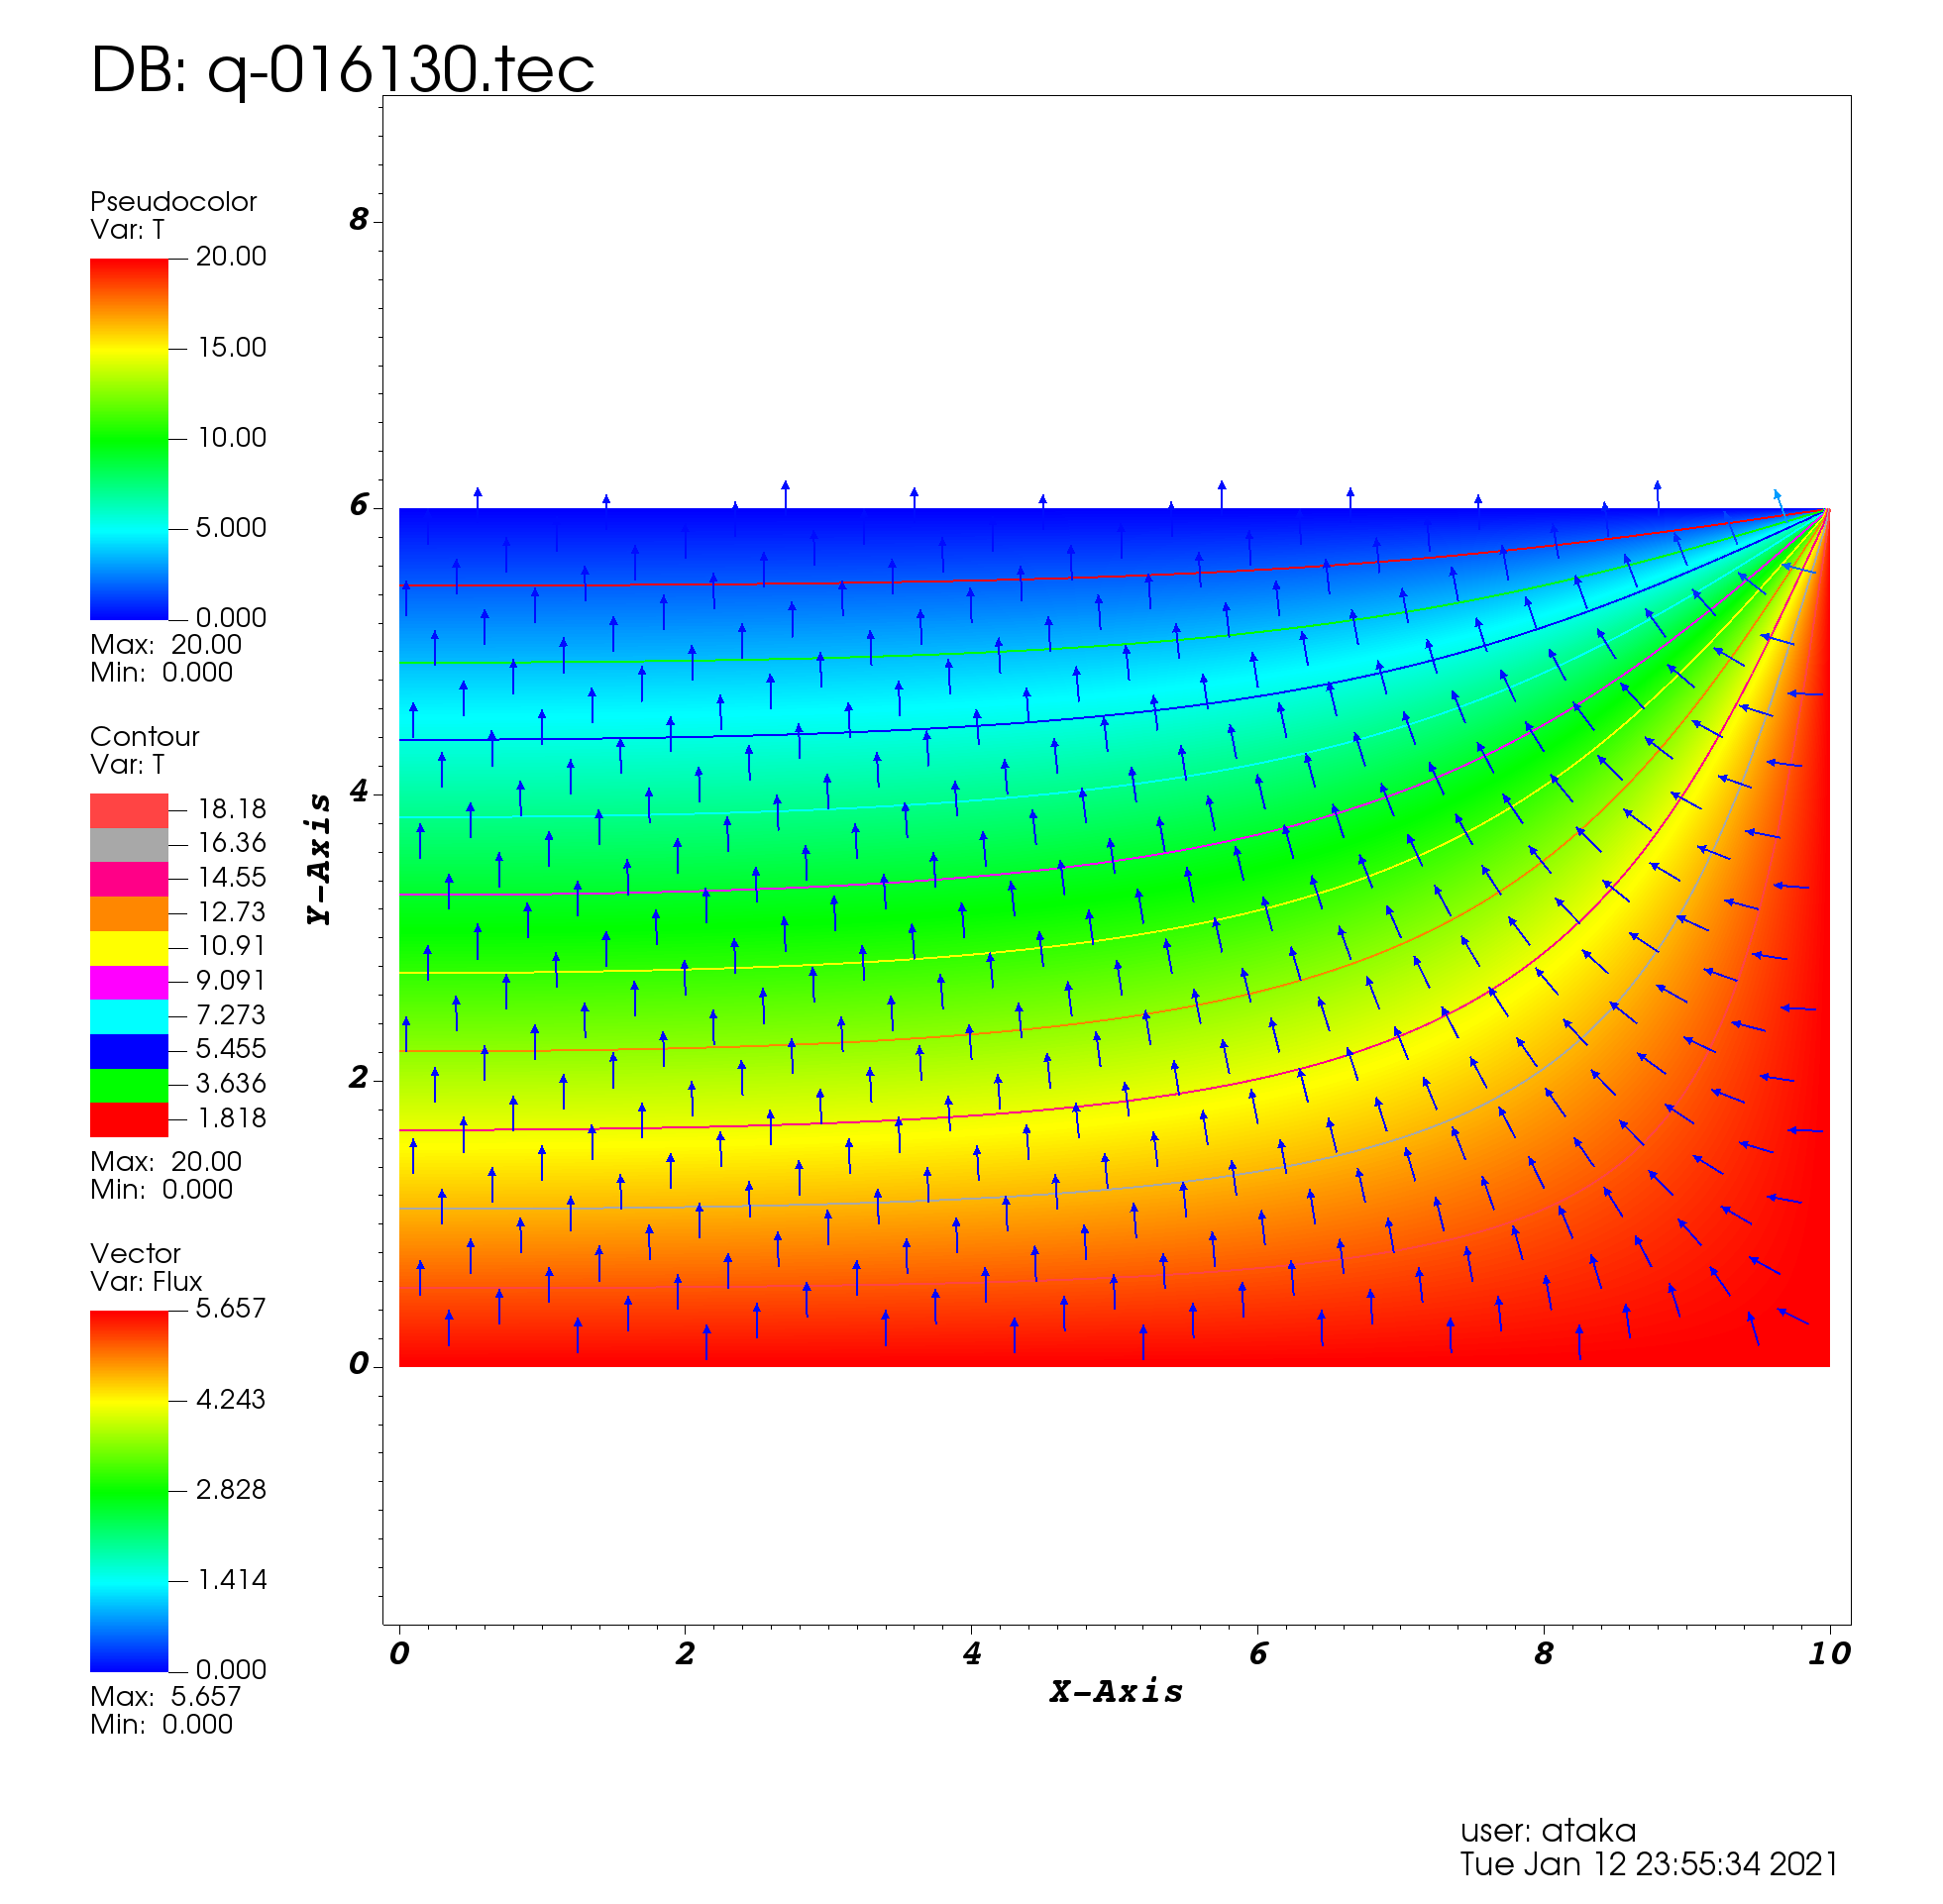
\includegraphics[max height=12cm]{graphs/gauss_norad/gauss_norad.png}
	\caption{Solution of the heat equation by Gauss-Seidel method.}
 	\label{fig:gaussnorad}
\end{figure}
\begin{figure}[H] 
	\centering 
	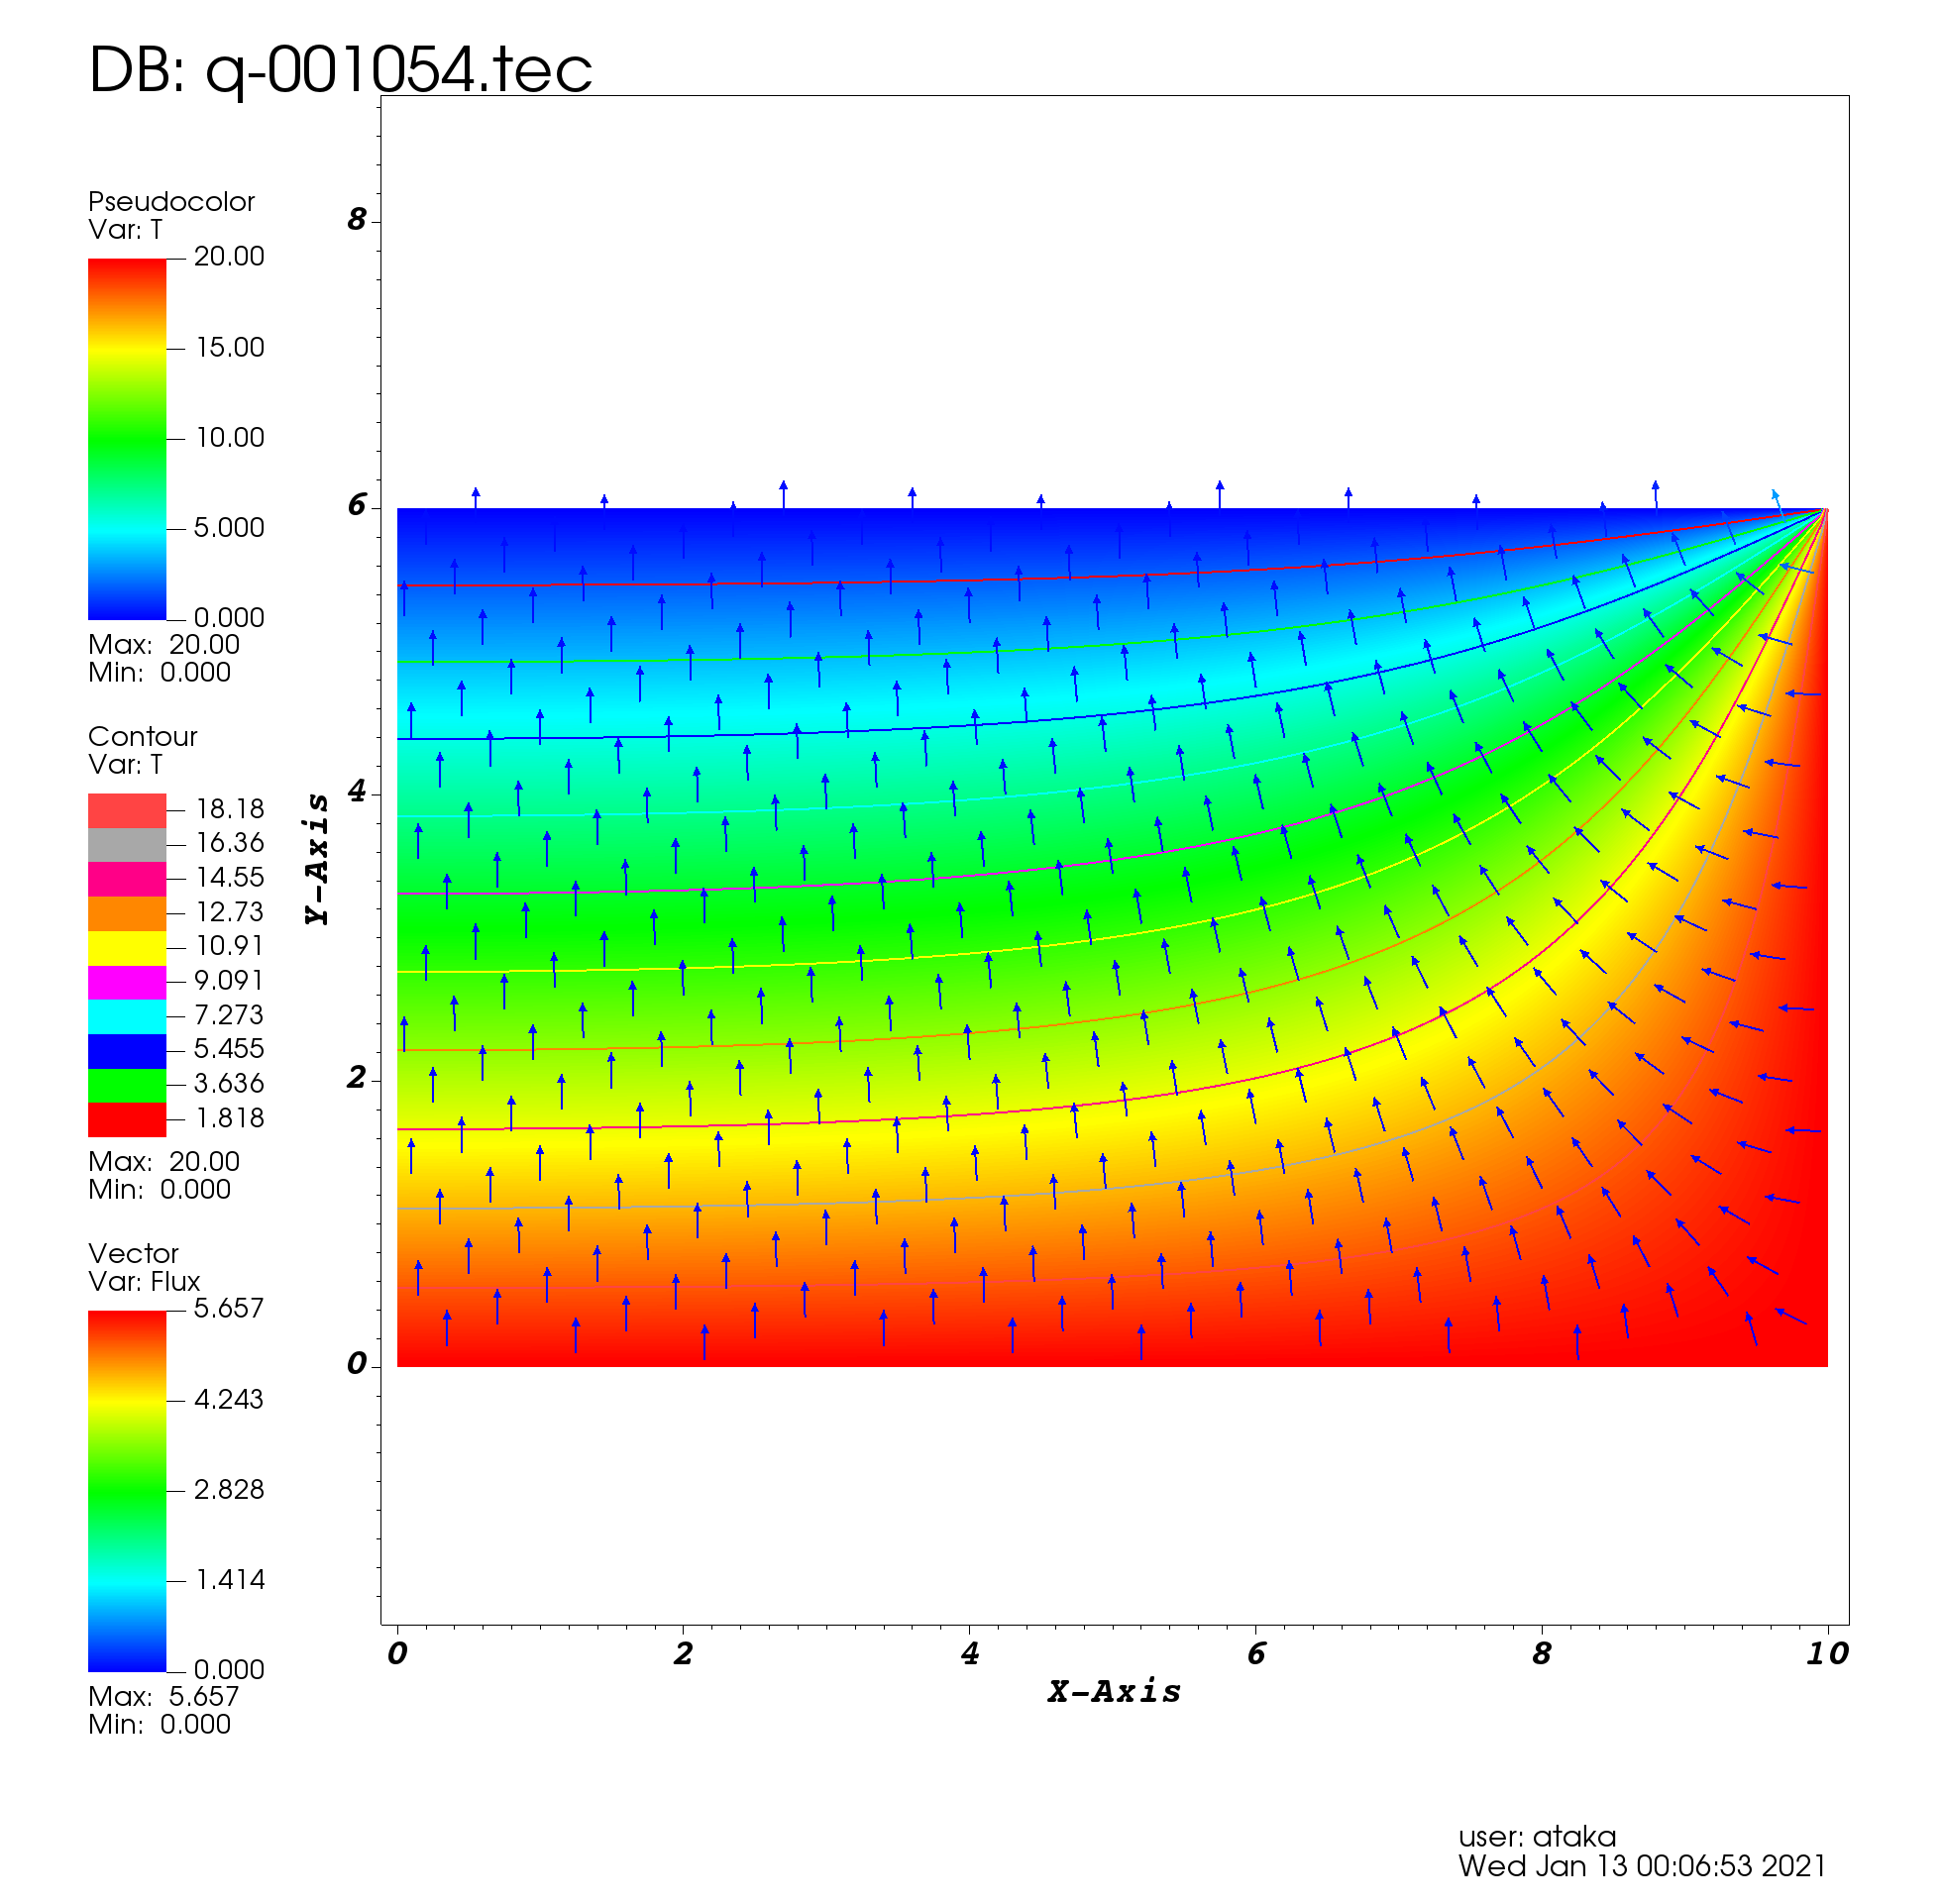
\includegraphics[max height=12cm]{graphs/SOR_O19_norad/SOR_O19_norad.png}
	\caption{Solution of the heat equation by SOR method.}
 	\label{fig:sornorad}
\end{figure}

\subsubsection{Temperature Distributions along x=5m and y=3m}
Figures \ref{fig:x5norad} and \ref{fig:y3norad} shows the temperature distributions along
x=5 and y=3 lines respectively. It can be oberved that all methods gave the same result with
a negligible difference among them although their convergence rates differ.  
\begin{figure}[H] 
	\centering 
	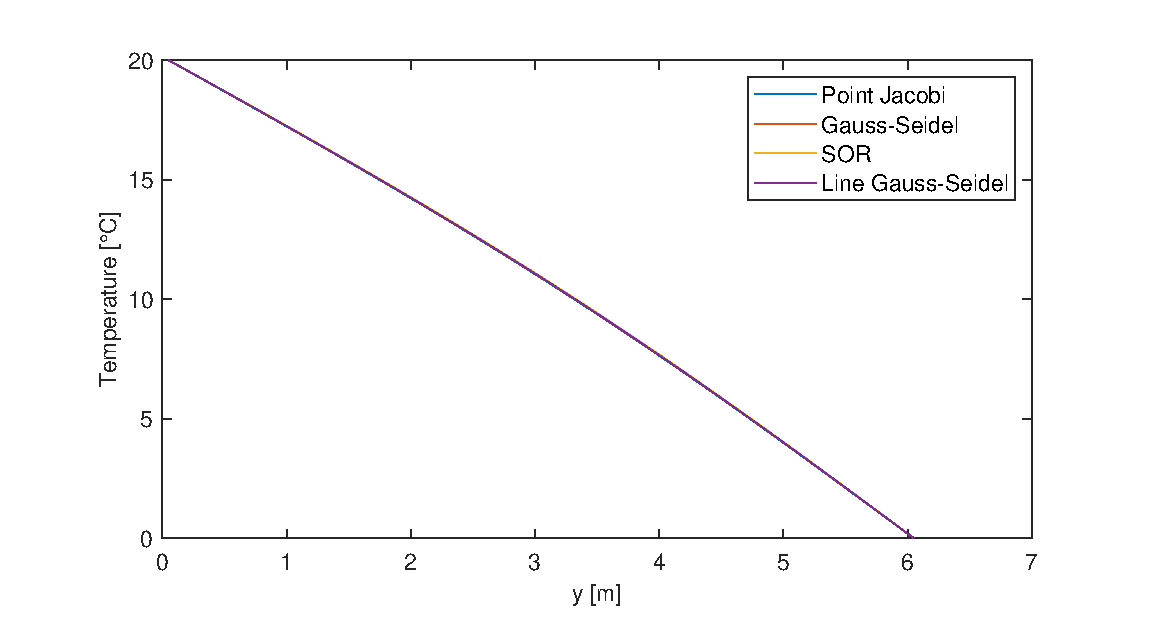
\includegraphics[max height=9cm]{graphs/x5_SOR19_norad.eps}
	\caption{Temperature distributions along x=5m}
 	\label{fig:x5norad}
\end{figure}
\begin{figure}[H] 
	\centering 
	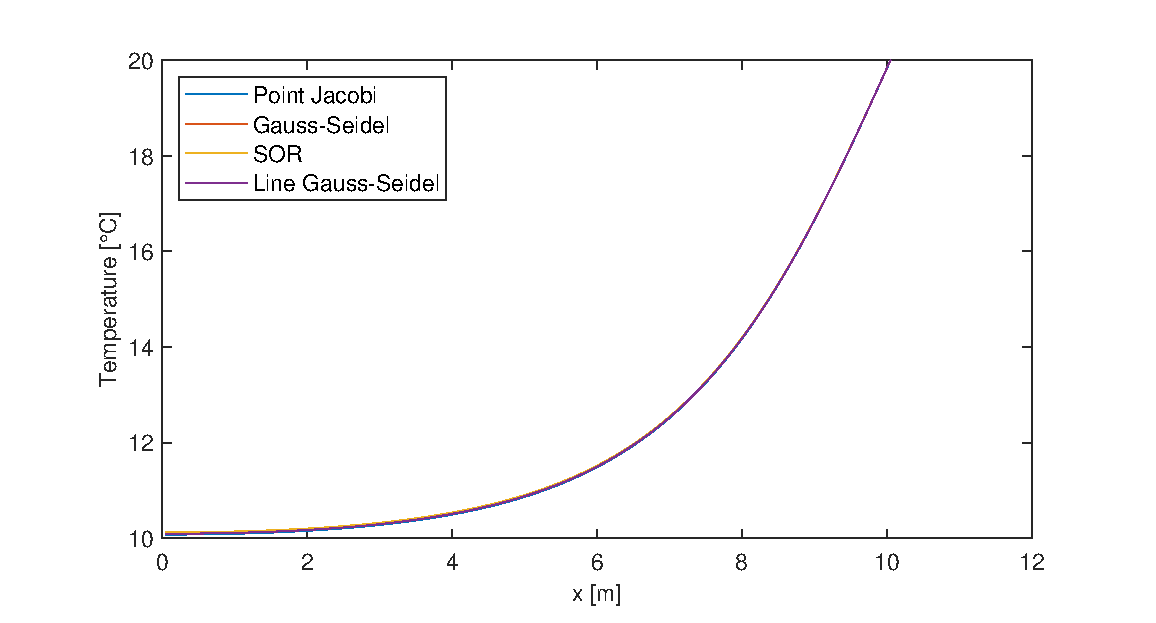
\includegraphics[max height=9cm]{graphs/y3_SOR19_norad.eps}
	\caption{Temperature distributions along y=3m}
 	\label{fig:y3norad}
\end{figure}

\subsection{Solution of the Heat Equation with Existence of a Radiator}
\begin{figure}[H] 
	\centering 
	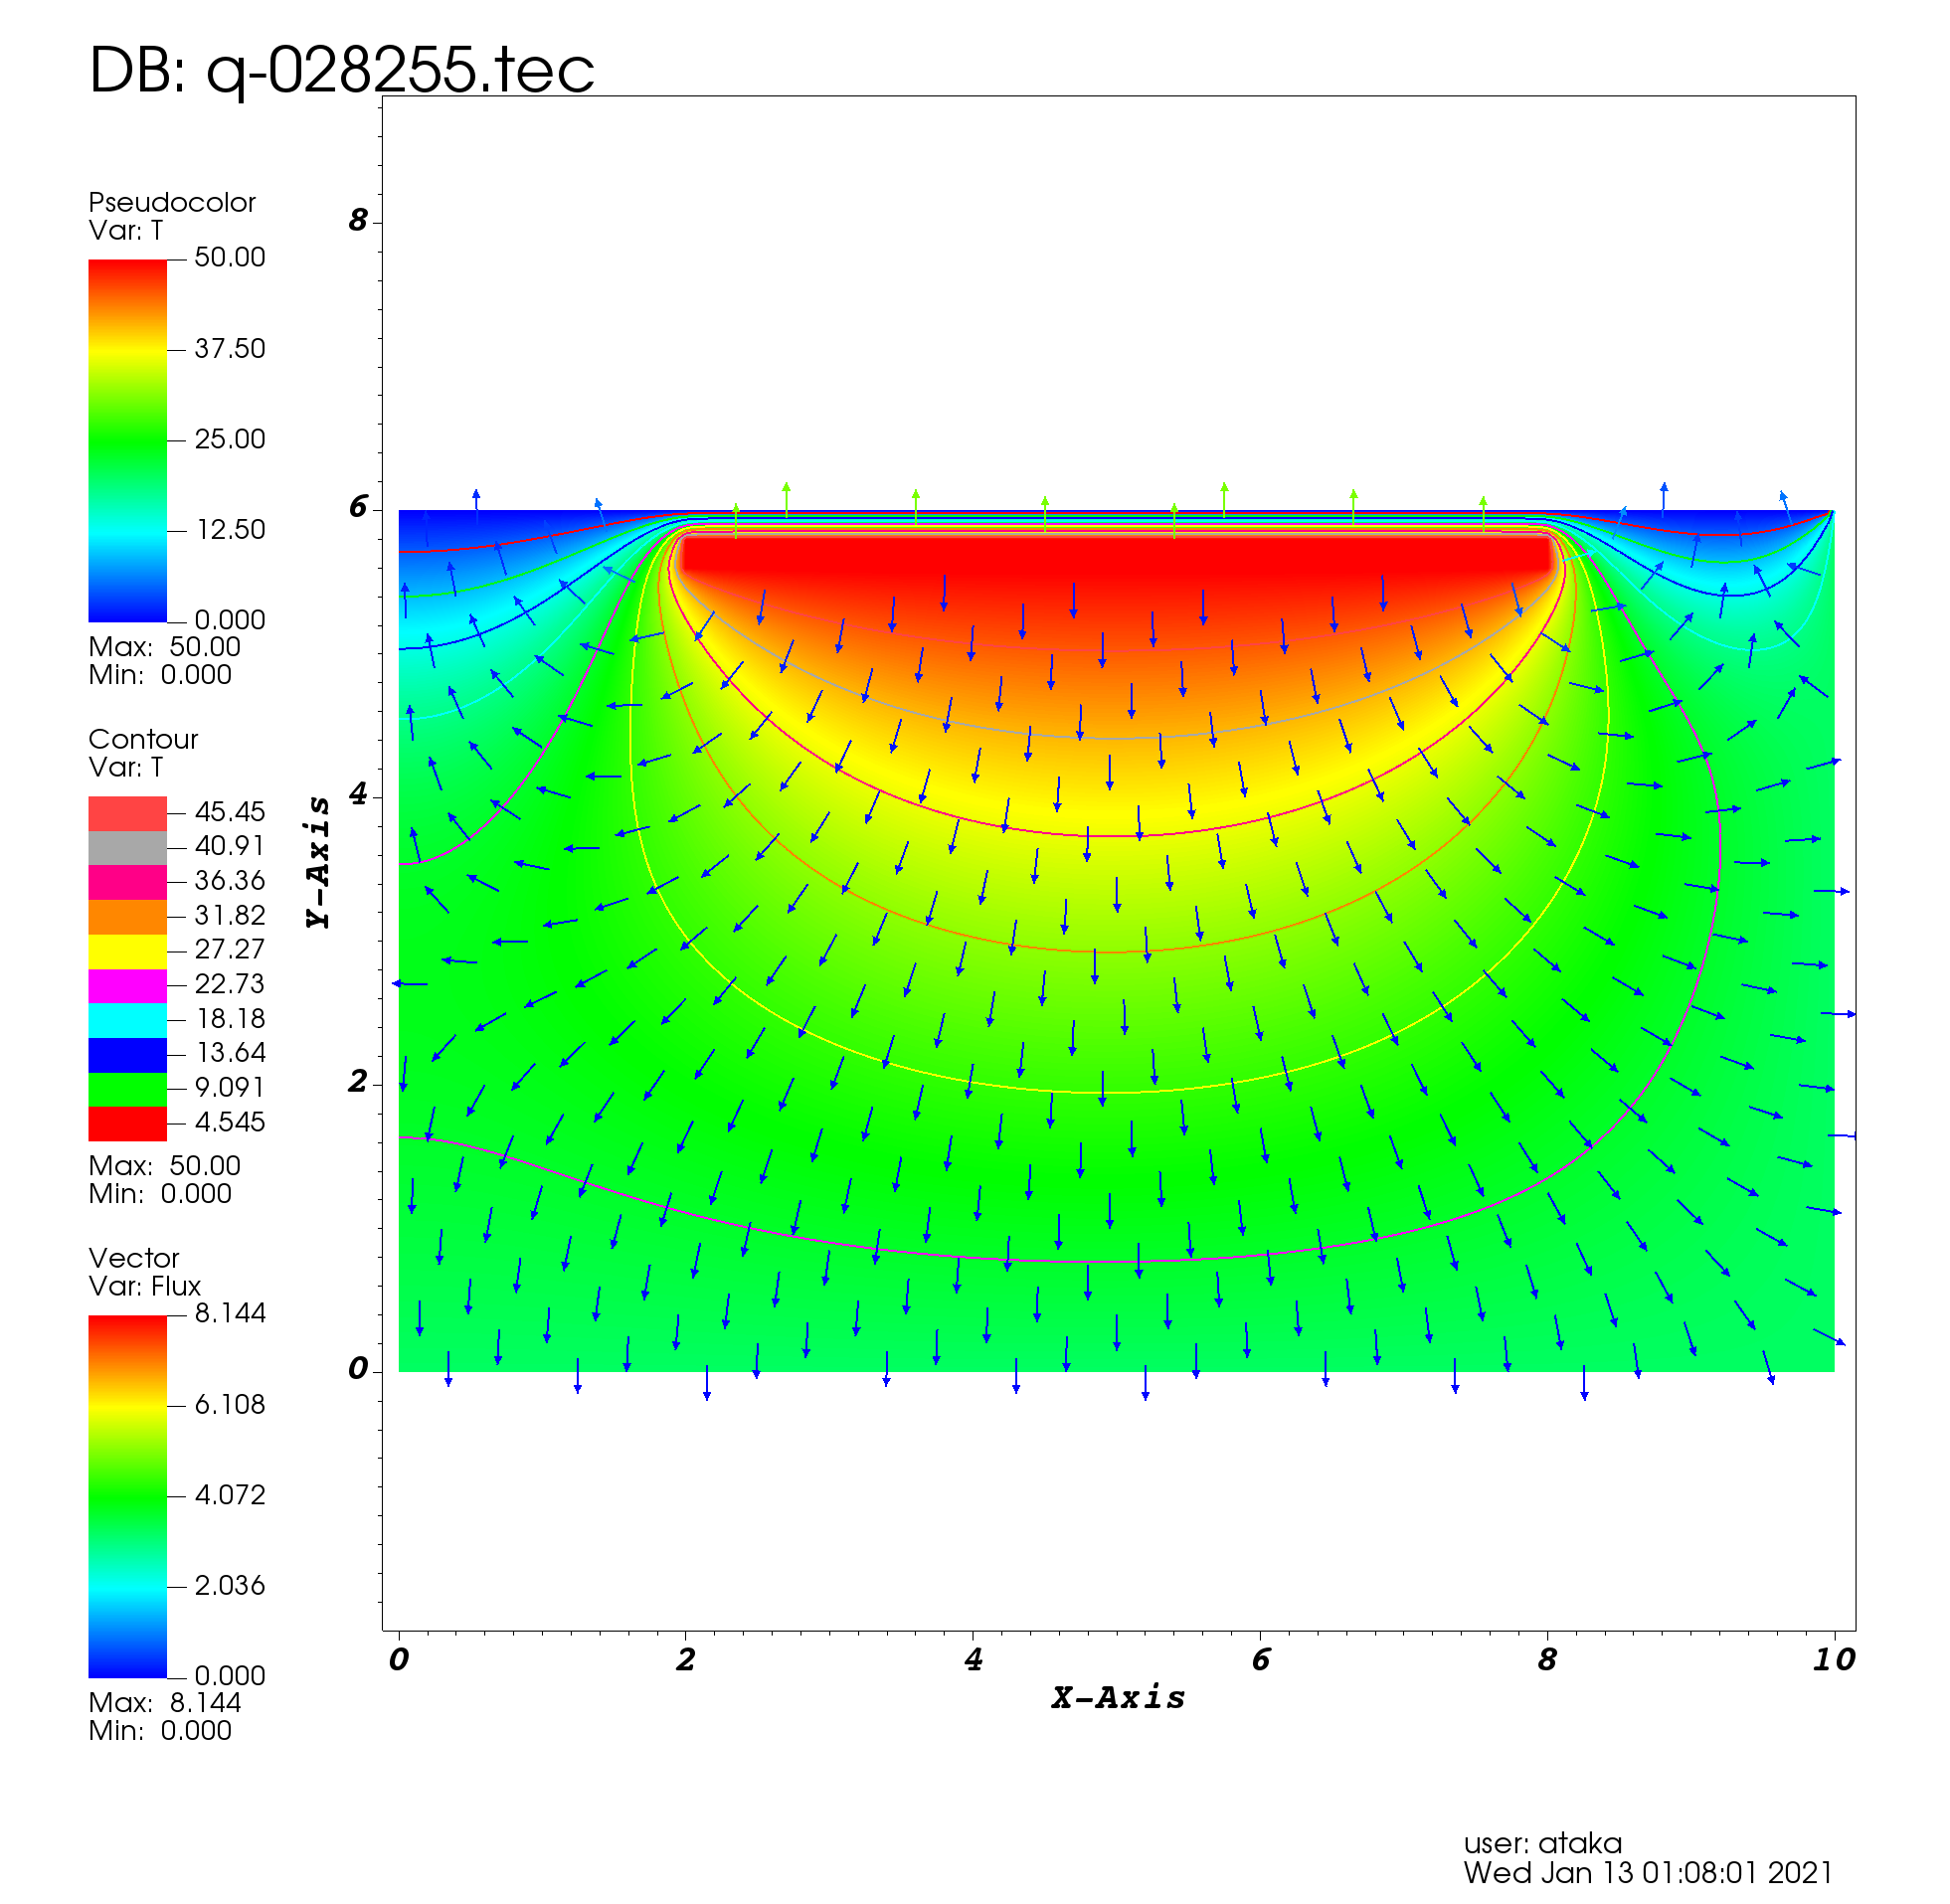
\includegraphics[max height=12cm]{graphs/point_rad_default/point_rad_default.png}
	\caption{Solution of the heat equation by Point Jacobi method.}
 	\label{fig:pointrad}
\end{figure}
\begin{figure}[H] 
	\centering 
	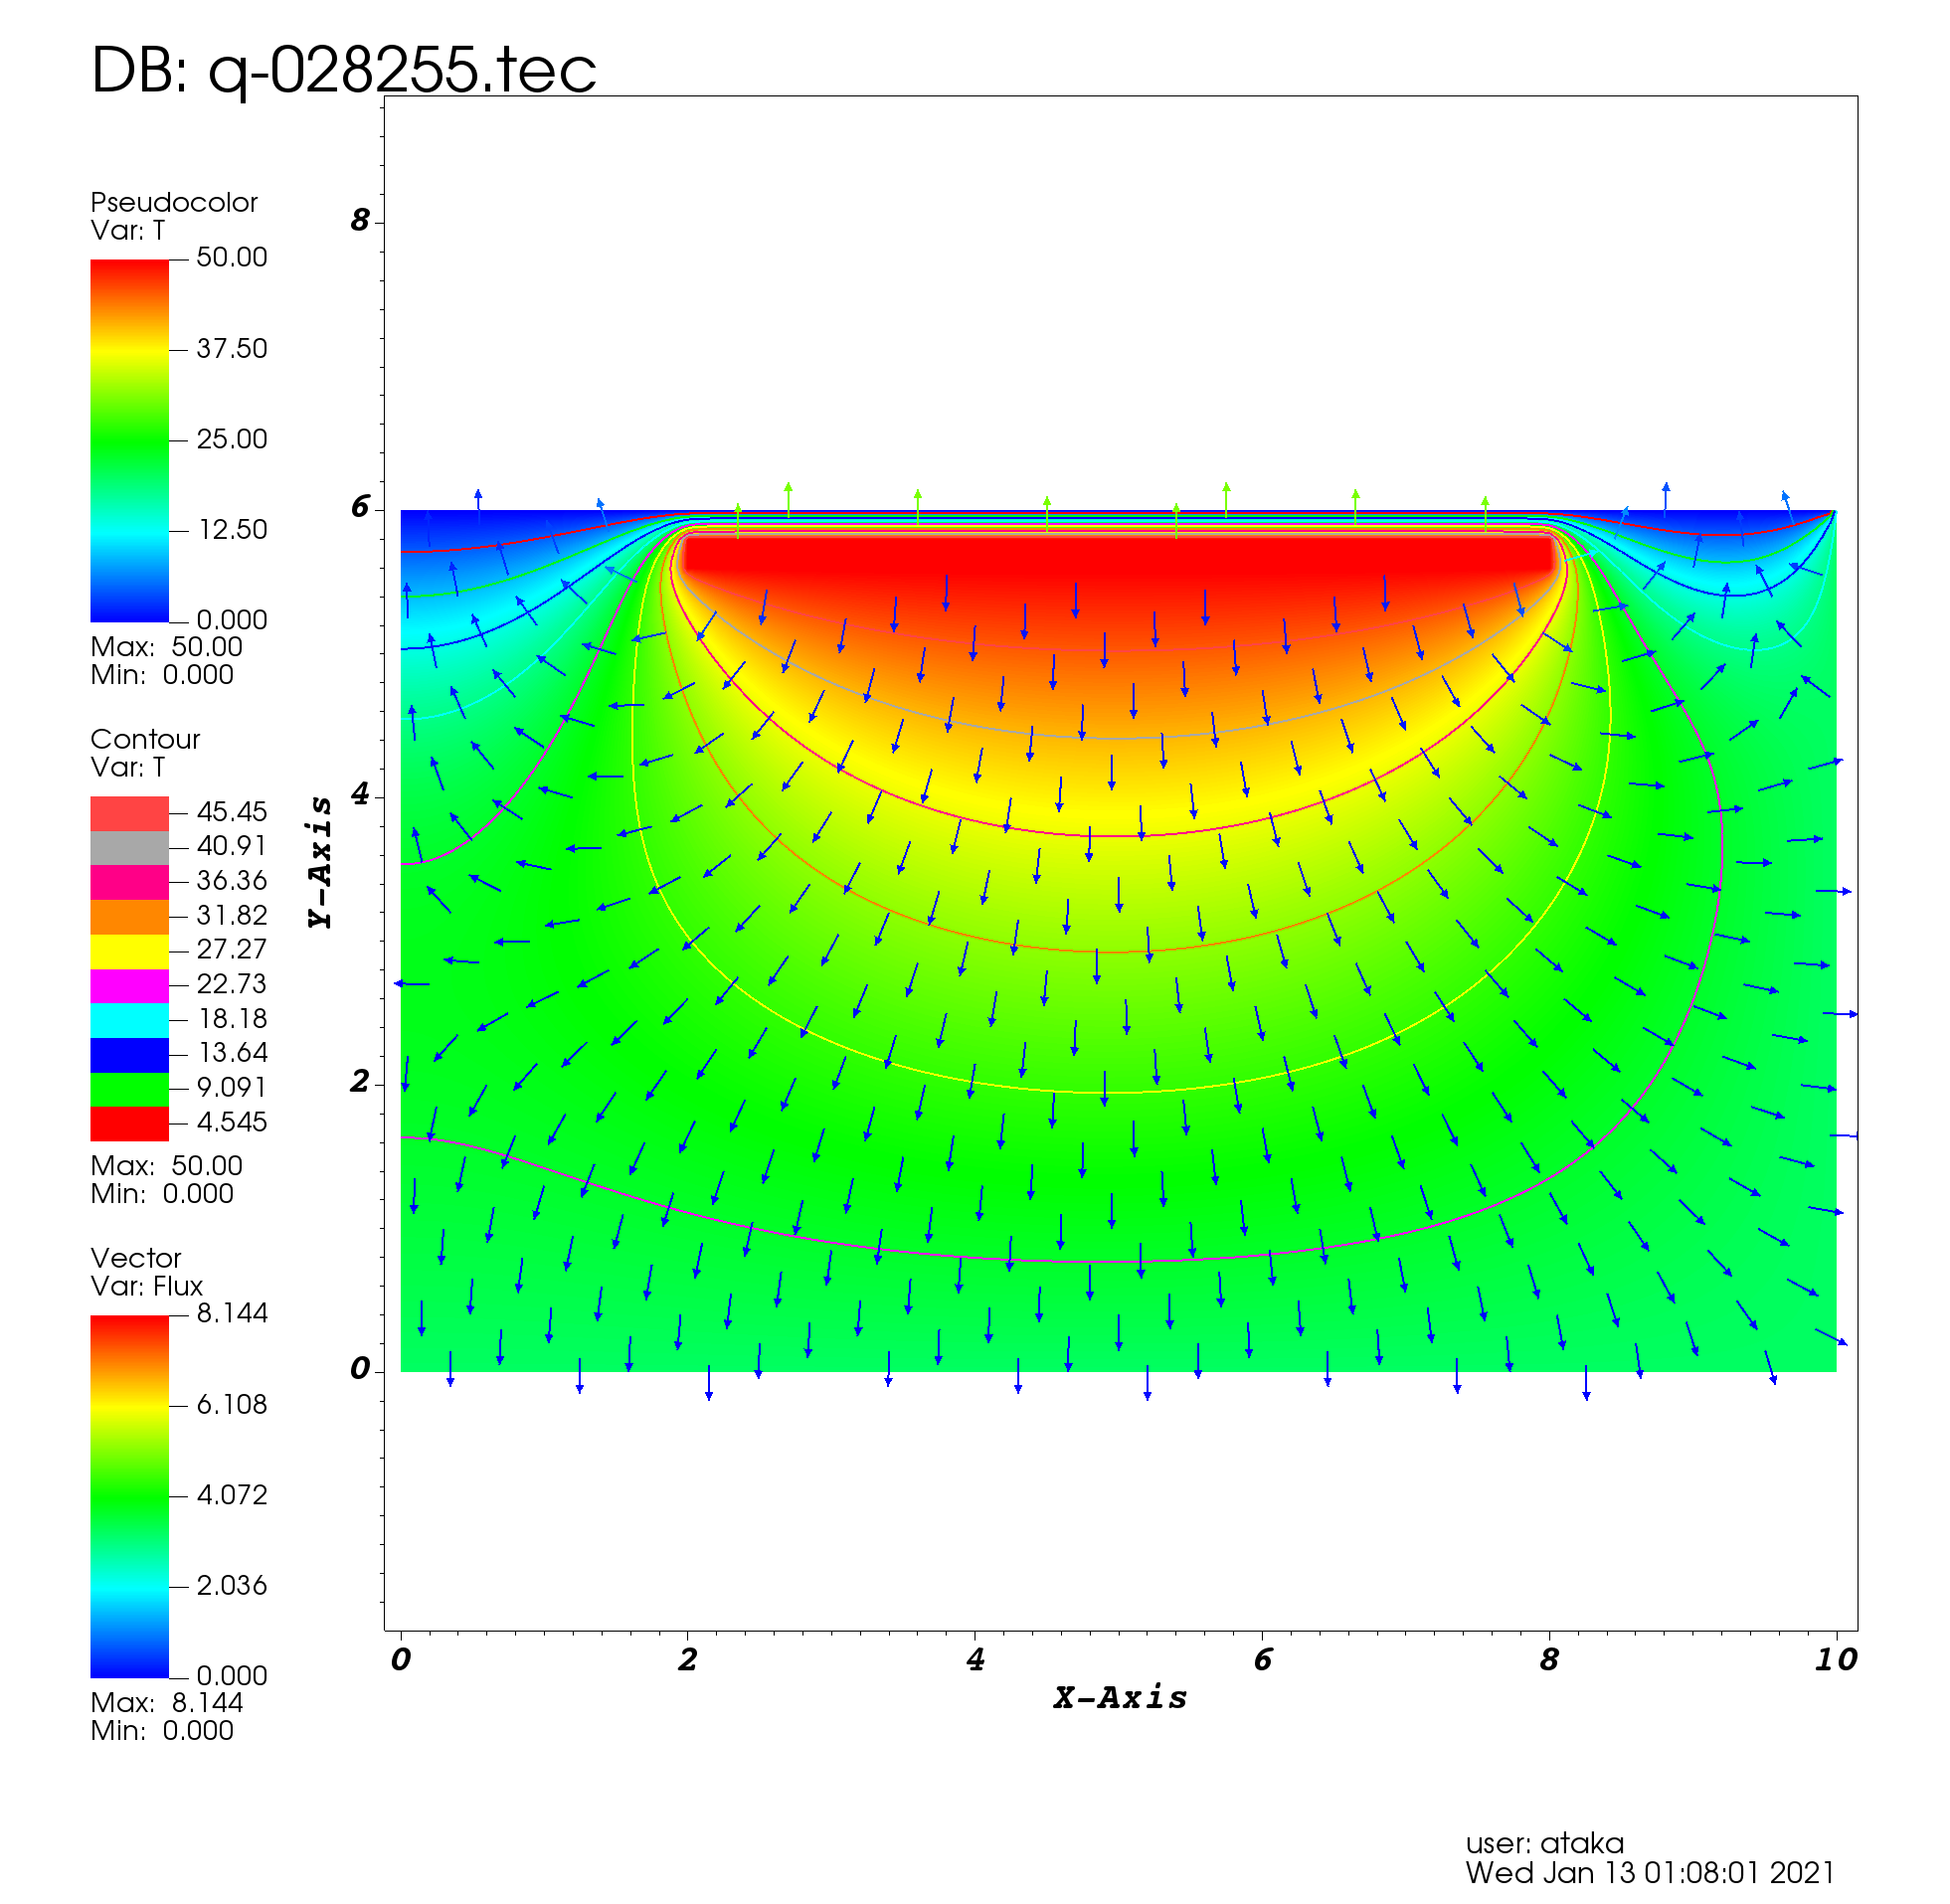
\includegraphics[max height=12cm]{graphs/gauss_rad_default/gauss_rad_default.png}
	\caption{Solution of the heat equation by Gauss-Seidel method.}
 	\label{fig:gaussrad}
\end{figure}
\begin{figure}[H] 
	\centering 
	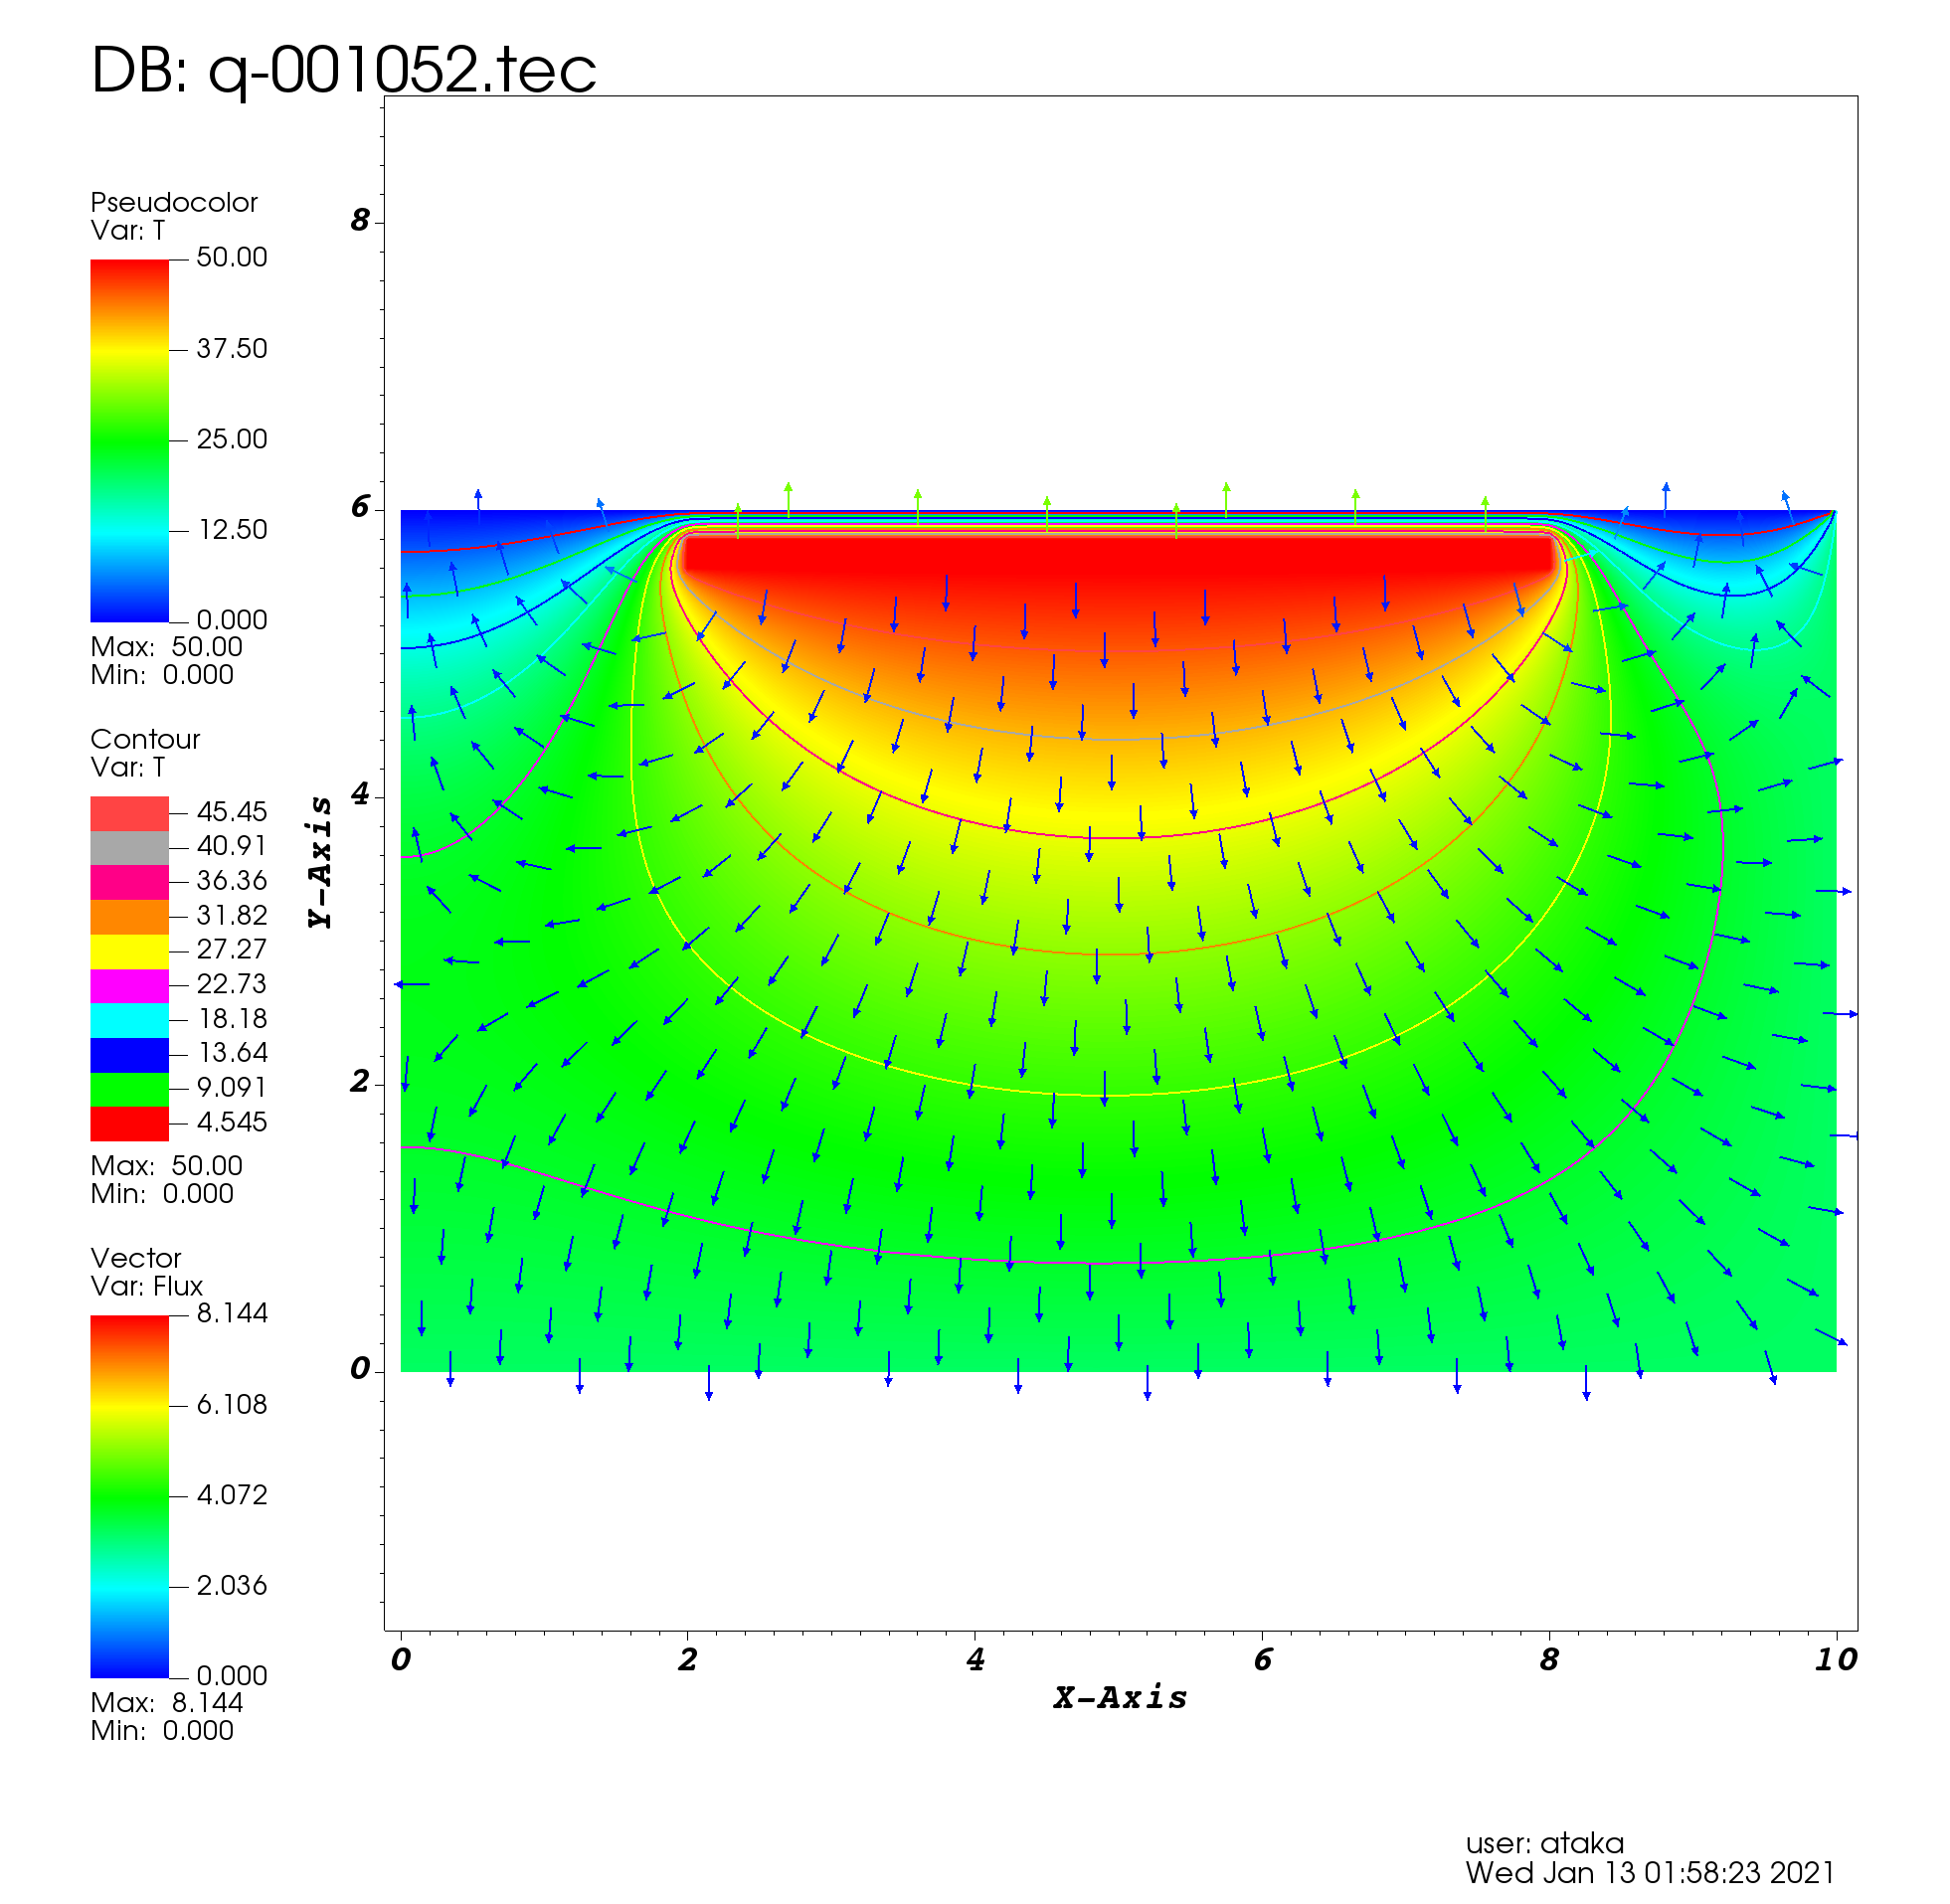
\includegraphics[max height=12cm]{graphs/SOR_O19_rad_default/SOR_O19_rad_default.png}
	\caption{Solution of the heat equation by SOR method.}
 	\label{fig:sorrad}
\end{figure}
Figures \ref{fig:pointrad}, \ref{fig:gaussrad}, and \ref{fig:sorrad}
demonstrates the solution of the heat equation by using Point Jacobi, Gauss-Seidel,
and SOR methods, respectively.From these figures, it can be observed that all the solutions
with different methods converged to nearly the same heat flux distributions.
In all solutions, the directions of the flux vectors are from the highest temperature surface
,which is the radiator, to the lower temperature surfaces, which is the walls of the room,
perpendicularly, except the insulated wall. Since the wall is insulated, the temperature
gradient across the wall is zero; hence the flux vectors are parallel near the surface.
Also, from the figures, it can be seen that all temperature contours which are intersect
with the insulated wall are perpendicular to the wall. Thus, it can said that heat transfer
does not occur from the room to the wall or reverse of it.

\subsubsection{Temperature Distributions along x=5m and y=3m}
\begin{figure}[H] 
	\centering 
	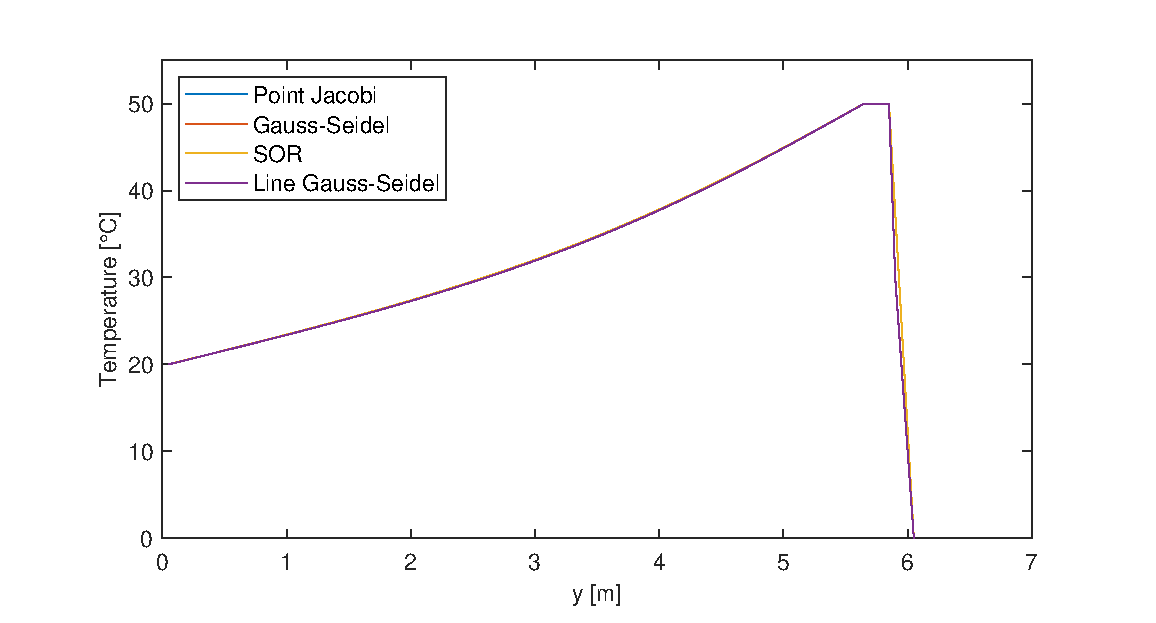
\includegraphics[max height=9cm]{graphs/x5_SOR19_defaultrad.eps}
	\caption{Temperature distributions along x=5m}
 	\label{fig:x5rad}
\end{figure}
\begin{figure}[H] 
	\centering 
	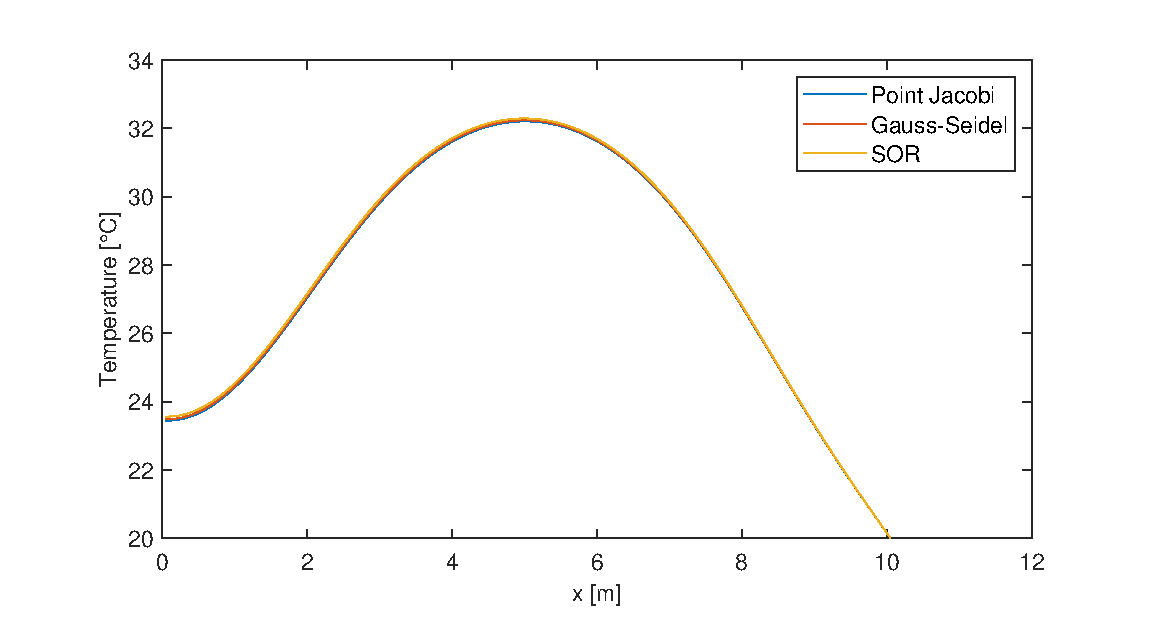
\includegraphics[max height=9cm]{graphs/y3_SOR19_defaultrad.eps}
	\caption{Temperature distributions along y=3m}
 	\label{fig:y3rad}
\end{figure}
Figures \ref{fig:x5rad} and \ref{fig:y3rad} illustrates the temperature distributions with the
existence of radiator along x=5m and y=3m lines, respectively. In Figure \ref{fig:x5rad}, sudden
change is observed near the y = 6m. The reason for this is that there is radiator between y = 5.6m
and 5.8m. Therefore, a sudden rise in temperature is seen before y=5.8 meters. This causes distortion
in both figures. However, in Figure \ref{fig:y3rad}, due to the the length of the radiator is 
longer in x-axis, its effect along y = 3m is less sudden.

\subsection{Comparison of the Convergence Rates}
Figures \ref{fig:convnorad} and \ref{fig:convrad} demonstrate the convergence rates of Point
Jacobi, Gauss-Seidel, and SOR methods for the solutions of the heat equation without and with
the radiator, respectively. As can be observed from these figure, the responses of Point Jacobi
method are the slowest. On the other hand, Gauss-Seidel method converges faster for both.
This is because it uses newly computed values of the unknowns as they become available as 
mentioned in Subsection ?. Furthermore, SOR method computed the solutions with minimum number
of iterations which is a result of the use of the relaxation parameter. This is also mentioned
in Subsection ?. The relaxation parameter is taken 1.9 for both since this is its largest
possible value which is found experimentally. For higher relaxation parameter values, the
solutions did not converge.

\begin{figure}[H] 
	\centering 
	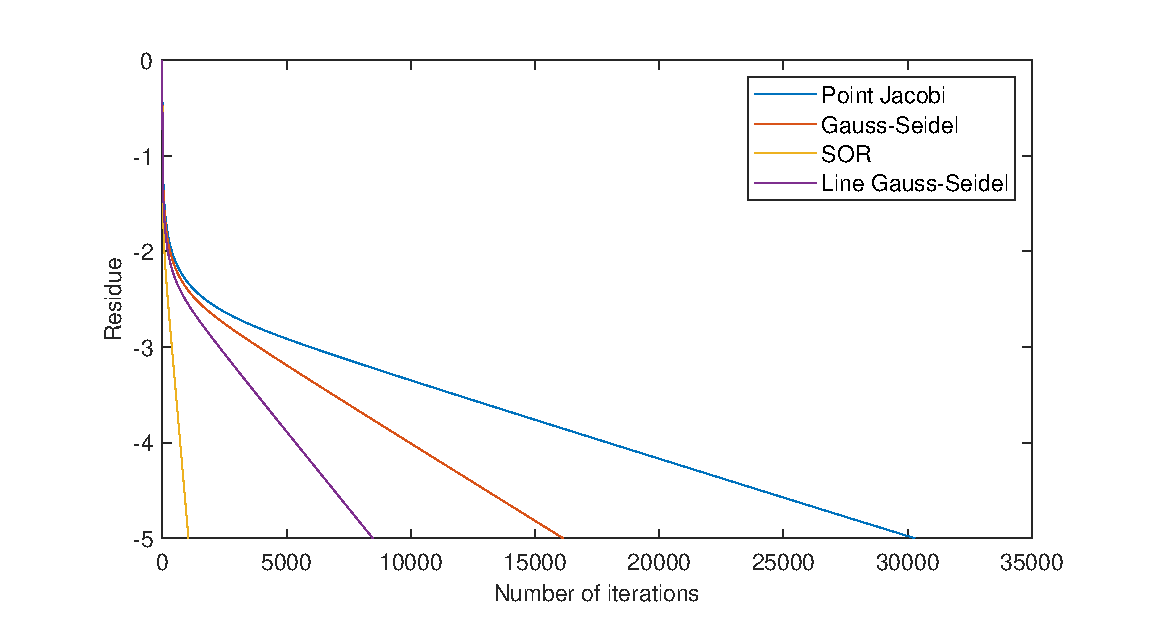
\includegraphics[max height=9cm]{graphs/residual_SOR19_norad.eps}
	\caption{Convergence rates of Point Jacobi, Gauss-Seidel and SOR methods in the absence of the radiator.}
 	\label{fig:convnorad}
\end{figure}

\begin{figure}[H] 
	\centering 
	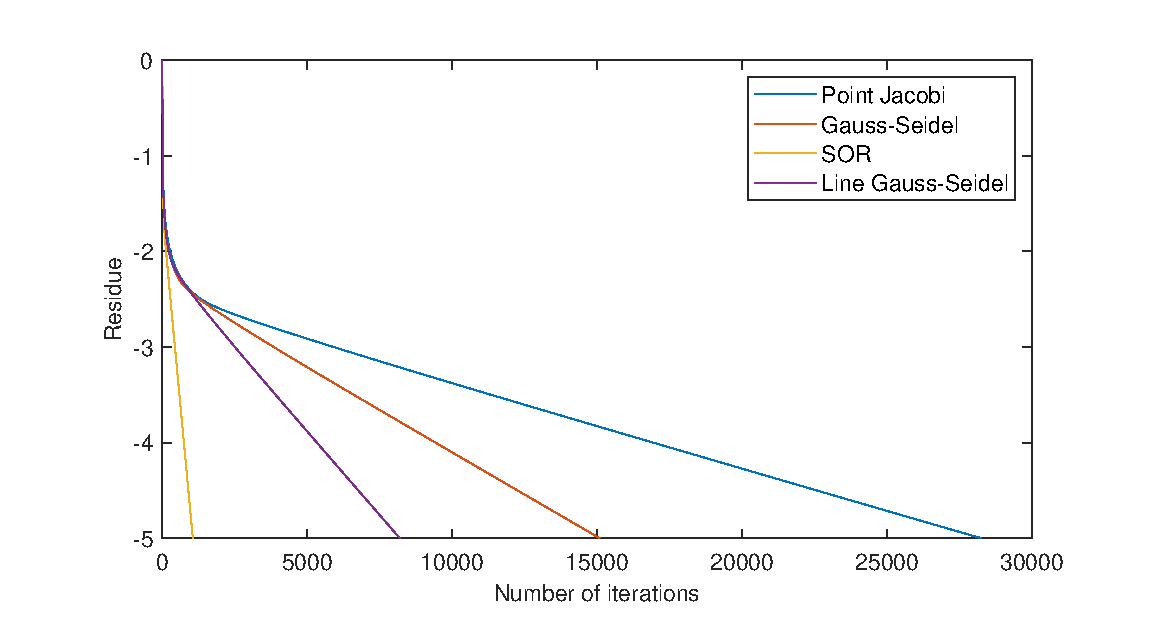
\includegraphics[max height=9cm]{graphs/residual_SOR19_defaultrad.eps}
	\caption{Convergence rates of Point Jacobi, Gauss-Seidel and SOR methods in the presence of the radiator.}
 	\label{fig:convrad}
\end{figure}

\section{Conclusion}
\end{document}